\documentclass[preprint,12pt]{elsarticle}
% Robotics and Autonomous Systems (Elsevier) -- manuscript source.
% Figures and tables are generated by figures/source_code/make_figures.py and tables/source_code/make_tables.py
% from the original records; see FIGURE_PROVENANCE.json and TABLE_PROVENANCE.json.

\usepackage{amsmath,amssymb}
\usepackage{graphicx}
\usepackage{booktabs,multirow,array}
\usepackage[hidelinks]{hyperref}
\usepackage{lineno}
\usepackage{xcolor}
\graphicspath{{./}}
\newcommand{\tabdir}{}
\renewcommand{\Pr}{\operatorname{P}}
\newcommand{\Bin}{\operatorname{Bin}}
\linenumbers

\journal{Robotics and Autonomous Systems}

\begin{document}

\begin{frontmatter}

\title{When Recovery Hurts: Separating Rescue from Harm in an Observation-Only Recovery Intervention for a Frozen Visuomotor Policy}

% AUTHOR ITEMS TO CONFIRM: name spelling, affiliation, e-mail, ORCID (see editorial/author_items_to_confirm.md)
\author[1]{[Author name to confirm]}
\ead{[corresponding e-mail to confirm]}
\affiliation[1]{organization={[Affiliation to confirm]},
            country={[Country to confirm]}}

\begin{abstract}
Recovery interventions on frozen robot policies are usually judged by the failures they repair. The same intervention can also turn an episode that the policy would have completed into a failure, and an average success gain hides that second effect. We study this for a diffusion policy that stacks cubes in simulation. At the moment the policy is about to release the held cube, an observation-only controller (Vision-CENTER V2) estimates the horizontal offset between the two cubes from a base and a wrist RGB camera and a short visual memory, and either abstains or makes a bounded horizontal move before handing control back. Each scene is branched from one simulator snapshot, so intervened and uninterrupted runs are paired, and we count rescues (failure to success) and harms (success to failure) separately. After development, two pre-registered confirmatory stages used new scenes. On 400 calibration scenes per policy, harm was 1 of 348 and 0 of 337 baseline successes, and an exact binomial test with Holm correction rejected a conditional harm rate above 5\% for both policies ($\delta=0.05$). On 400 held-out test scenes per policy, run once, success rose from 350 to 379 and from 347 to 373 (29 rescues vs 0 harms, $p=1.9\times10^{-9}$; 27 vs 1, $p=1.1\times10^{-7}$). We also report a failed physics-validity check, a memory ablation and a second policy architecture. The certificate is statistical and task-level; it is not a physical safety guarantee.
\end{abstract}

\begin{keyword}
recovery intervention \sep frozen visuomotor policy \sep paired evaluation \sep outcome harm \sep finite-sample certificate \sep diffusion policy \sep robotic manipulation
\end{keyword}

\end{frontmatter}

%% ---------------------------------------------------------------------------------------------------------
\section{Introduction}\label{sec:intro}

Learned visuomotor policies such as diffusion policies \cite{chi2023diffusion} are increasingly deployed as frozen components: after training, their weights are fixed, and any further improvement must come from outside the network. A natural outside improvement is a runtime recovery intervention: a monitor decides that something is about to go wrong, a small controller corrects the state, and the policy resumes. Many methods of this kind exist, from learned recovery policies \cite{reichlin2022manifold,cideron2023getback,vats2025recoverychaining} to human or learned interventions during interactive imitation \cite{ross2011dagger,kelly2019hgdagger,hoque2022thrifty} and runtime failure monitors \cite{agia2025unpacking,romer2025fiper,liu2023reflect,duan2025aha}.

An intervention on a frozen policy changes the state from which the policy continues. If the policy would have failed, the change can rescue the episode. If the policy would have succeeded, the same change can also cause a failure, for example by spending the time budget or by moving the gripper into a configuration the policy handles badly. The net change in success rate is the number of rescues minus the number of harms, so an intervention with many rescues and many harms looks as good as one with fewer rescues and no harm. The two have different consequences for a user who already relies on the policy's successes, so we report them separately.

This paper asks one question. \emph{Can an observation-only recovery intervention on a frozen policy increase task success while keeping, with a finite-sample statistical guarantee, the rate at which it turns the policy's own successes into failures below a stated level?} We answer it for one task, one intervention and two independently trained policies, and we report every step of the argument, including the parts that did not work.

The study is built around three design choices.
\begin{enumerate}
\item \textbf{Paired branching.} Each scene runs once until the trigger; the simulator state is saved, and the uninterrupted policy (C0), the proposed controller and all ablations are run from that same snapshot. Each scene therefore yields a pair of outcomes $(Y_0, Y_g)$ and falls into one of four cells: both succeed, rescue, harm, both fail (Fig.~\ref{fig:problem}a).
\item \textbf{Harm as a conditional rate.} We define harm as $h(g)=\Pr(Y_g=0 \mid Y_0=1)$, the probability that the intervention $g$ turns a baseline success into a failure, and test $h(g)\le\varepsilon$ with an exact binomial test on calibration scenes that were not used for development.
\item \textbf{Separation of certificate and efficacy.} The harm certificate is computed on a calibration split; the efficacy claim (more successes than without the intervention) is tested once on a separate, held-out test split, under a frozen manifest.
\end{enumerate}

\begin{figure}[!htbp]
\centering
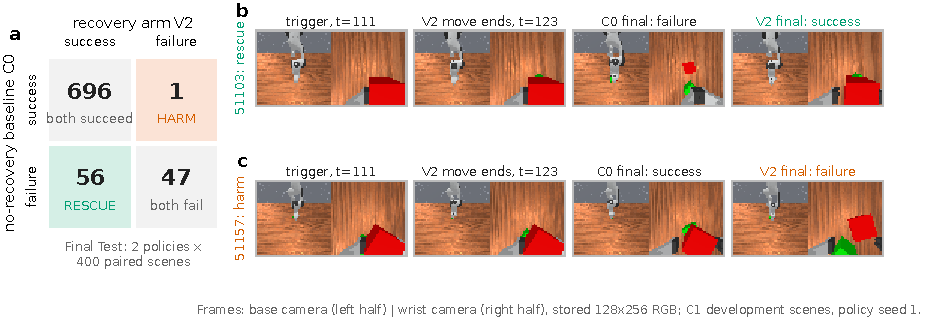
\includegraphics[width=\linewidth]{F1_problem_rescue_vs_harm.pdf}
\caption{Rescue and harm. (a) Paired outcome matrix of the Final Test, both policies. (b) A development rescue (scene 51103, policy seed 1): the policy alone fails; after the V2 move the policy's own release places the cube and the episode succeeds. (c) The only development harm of V2 for policy seed 1 (scene 51157): the policy alone drops the cube, regrasps it and succeeds at step 190; with V2 it fails. Each frame shows the stored base-camera (left half) and wrist-camera (right half) RGB images without processing.}\label{fig:problem}
\end{figure}

The contributions are the following.
\begin{itemize}
\item A paired evaluation protocol for recovery interventions on a frozen policy that reports rescue and harm separately and certifies the conditional harm rate with an exact finite-sample test (Section~\ref{sec:problem}).
\item Vision-CENTER V2, an observation-only release-time centring controller with a short visual memory and explicit abstention rules (Section~\ref{sec:method}).
\item A two-stage confirmatory result on 1,600 new paired scenes for two policies: the harm rate is certified below 5\% on calibration scenes, and the success gain is confirmed on held-out test scenes (Section~\ref{sec:confirm}).
\item A descriptive mechanism analysis that traces a representative rescue and the single development harm through observation, memory, decision, movement and hand-back, including a commanded-versus-actual motion audit of all moves (Section~\ref{sec:mechanism}).
\item An audit of the physical record that the analyses rely on. One of its checks, the agreement of logged contact separations with reconstructed gaps, fails; we report the failure, partially explain it, and state what it does and does not affect (Section~\ref{sec:physics}).
\end{itemize}

We do not claim physical safety, transfer to other tasks or to a real robot, or that the paired-branching design and the binomial certificate are new statistical ideas. Exact binomial bounds and risk-control procedures are well known \cite{clopper1934,angelopoulos2021ltt}; the contribution is their use to separate rescue from harm for a recovery intervention, together with a descriptive mechanism analysis of the controller. The controller itself is task-specific; we present it as a case study for the evaluation protocol, which is the part we expect to transfer.

%% ---------------------------------------------------------------------------------------------------------
\section{Related work}\label{sec:related}

\paragraph{Recovery for learned policies}
Learned policies drift away from the states seen in demonstrations, and the resulting compounding error is the classical motivation for interactive imitation learning \cite{ross2011dagger,laskey2017dart}. Recovery methods return the system to familiar states: Back to the Manifold learns to steer out-of-distribution states back to the data manifold \cite{reichlin2022manifold}, POIR plans a return to the demonstration distribution \cite{cideron2023getback}, RecoveryChaining learns local recovery policies that hand control back to a nominal controller \cite{vats2025recoverychaining}, and Recovery RL restricts exploration with a learned recovery policy \cite{thananjeyan2021recoveryrl}. Recent work on vision--language--action and world--action models adds recovery at scale \cite{liufu2026repovla,li2026causalhistory}, retries after failure \cite{du2024toerr}, or rewinds to an earlier state \cite{zheng2026rewind}. These methods are usually evaluated by success rate with and without recovery; our concern is the decomposition of that difference into rescues and harms on paired states.

\paragraph{Interventions and runtime monitoring}
Interactive imitation learning lets a human or a gate decide when to intervene \cite{kelly2019hgdagger,hoque2022thrifty}. Runtime monitors detect failures of generative policies from consistency and progress \cite{agia2025unpacking} or predict them online \cite{romer2025fiper}; language-model systems explain and correct failures \cite{liu2023reflect,duan2025aha}; CheckVLA verifies action chunks with a world model \cite{liu2026checkvla}. A failure prediction does not say whether acting on it helps. RESCUE makes exactly this point and evaluates monitor alarms by counterfactual interventions from the same policy state \cite{ahmedt2026rescue}, and a recent study audits whether memory in history-conditioned policies actually guides decisions \cite{zhang2026memory}. Our evaluation shares the counterfactual, same-state view; it adds a pre-registered confirmatory split and a certificate on the harm side.

\paragraph{Statistical risk control}
Learn then Test calibrates algorithms so that a chosen risk is controlled with finite-sample guarantees through multiple testing \cite{angelopoulos2021ltt}. Our certificate is the simplest instance of this idea: a single, pre-specified candidate and one binomial test per policy, combined with Holm's procedure \cite{holm1979}. The efficacy test is the exact one-sided form of McNemar's paired test \cite{mcnemar1947}.

Table~\ref{tab:related} positions the present work against the closest papers. The table describes what each paper evaluates as stated in that paper; it is not a ranking.

\begin{table}[!htbp]
\centering\footnotesize
\caption{Positioning against related work (qualitative; based on each paper's own description).}\label{tab:related}
\begin{tabular}{p{0.24\linewidth}p{0.30\linewidth}p{0.38\linewidth}}
\toprule
Work & Primary question & Difference from this paper\\
\midrule
DAgger, DART, HG-DAgger, ThriftyDAgger \cite{ross2011dagger,laskey2017dart,kelly2019hgdagger,hoque2022thrifty} & collect corrective data or gate human interventions during training & the policy here is frozen; interventions are evaluated, not used for training\\
Back to the Manifold, POIR, RecoveryChaining, Recovery RL \cite{reichlin2022manifold,cideron2023getback,vats2025recoverychaining,thananjeyan2021recoveryrl} & learn a recovery behaviour & our controller is hand-designed and bounded; we separate its rescues from its harms on paired states\\
Sentinel, FIPER, REFLECT, AHA, CheckVLA \cite{agia2025unpacking,romer2025fiper,liu2023reflect,duan2025aha,liu2026checkvla} & detect, predict or explain failures & we evaluate what an action taken at the trigger does to the outcome\\
RESCUE \cite{ahmedt2026rescue} & is an alarm worth acting on? counterfactual interventions from the same state & we add a calibration certificate for harm and a held-out confirmatory test\\
To Err is Robotic, Rewind-IL, RePO-VLA, Causal-History TTS \cite{du2024toerr,zheng2026rewind,liufu2026repovla,li2026causalhistory} & retry, rewind or optimise for recovery & we report conditional harm on baseline successes, not only success rate\\
Learn then Test \cite{angelopoulos2021ltt} & finite-sample risk control by multiple testing & we apply its simplest form to harm of one frozen candidate\\
\bottomrule
\end{tabular}
\end{table}

%% ---------------------------------------------------------------------------------------------------------
\section{Problem formulation}\label{sec:problem}

\paragraph{Research question} Given a frozen policy $\pi$ and an intervention $g$ that may act once per episode, does $g$ increase the success probability while keeping the probability that it destroys a success of $\pi$ below $\varepsilon$?

\paragraph{Paired outcomes} A scene $s$ is drawn from a seed distribution $\mathcal{D}$. The policy runs from the initial state until a trigger time $t^\star(s)$, determined only by the policy's own commands (Section~\ref{sec:method}). The full simulator state at $t^\star$ is saved. From that snapshot we run the policy unchanged, which gives $Y_0(s)\in\{0,1\}$, and the policy with intervention $g$, which gives $Y_g(s)\in\{0,1\}$. Scenes without a trigger have $Y_g=Y_0$ by construction. The four cells are
\begin{equation}
\begin{aligned}
\text{rescue}: &\ Y_0=0,\ Y_g=1, & \qquad \text{harm}: &\ Y_0=1,\ Y_g=0,\\
\text{both succeed}: &\ Y_0=1,\ Y_g=1, & \qquad \text{both fail}: &\ Y_0=0,\ Y_g=0.
\end{aligned}
\end{equation}
With $R$ rescues and $H$ harms on $n$ scenes, the change in the number of successes is $\sum_s (Y_g-Y_0)=R-H$.

\paragraph{Conditional harm} We define
\begin{equation}
h(g) \;=\; \Pr_{s\sim\mathcal{D}}\bigl(Y_g(s)=0 \,\bigm|\, Y_0(s)=1\bigr).
\end{equation}
It is the probability that a success the policy would have achieved alone is lost because of $g$. It concerns the task outcome in the simulator; it does not measure collision, force or damage.

\paragraph{Harm certificate} On $n$ calibration scenes drawn independently from $\mathcal{D}$ (we treat distinct scene seeds as independent draws; Supplementary Section~S1), let $n_+=\sum_s Y_0(s)$ and $k=\sum_s Y_0(s)\,(1-Y_g(s))$. Conditional on $n_+$, the scenes with $Y_0=1$ are an i.i.d.\ sample from $\mathcal{D}$ conditioned on $Y_0=1$, so $k\sim\Bin(n_+, h(g))$. For the null hypothesis $H_0^{\mathrm{harm}}: h(g)>\varepsilon$ the exact p-value is
\begin{equation}\label{eq:cert}
p_{\mathrm{harm}} \;=\; \sum_{j=0}^{k}\binom{n_+}{j}\,\varepsilon^{j}(1-\varepsilon)^{n_+-j},
\end{equation}
and $g$ is certified for policy $\pi$ when $p_{\mathrm{harm}}$ is below its Holm threshold. For the two policies we use Holm's procedure with family-wise level $\delta$ \cite{holm1979}: sort the two p-values, compare the smaller with $\delta/2$ and, if rejected, the larger with $\delta$. Under the null, the probability of a false certificate for any member of the family is at most $\delta$. We pre-registered $\varepsilon=\delta=0.05$.

\paragraph{Efficacy test} On the held-out test scenes, let $b$ be the number of rescues and $c$ the number of harms. Under the null hypothesis that the intervention does not increase success, $\Pr(Y_0=0,Y_g=1)\le\Pr(Y_0=1,Y_g=0)$, and conditional on the $d=b+c$ discordant scenes the number of rescues is stochastically at most $\Bin(d,1/2)$. The exact one-sided p-value is
\begin{equation}\label{eq:eff}
p_{\mathrm{eff}} \;=\; \sum_{j=b}^{d}\binom{d}{j}2^{-d},
\end{equation}
the exact form of McNemar's paired test \cite{mcnemar1947}. Holm's procedure is applied over the two policies at $\alpha=0.05$.

\paragraph{Information constraint} The monitor and the controller may use only the robot's cameras, its proprioception and their own history. They may not read object poses from the simulator, the success flag or any future quantity. A privileged oracle that reads the true cube positions is reported only as a reference, never as a candidate.

%% ---------------------------------------------------------------------------------------------------------
\section{Vision-CENTER V2}\label{sec:method}

Figure~\ref{fig:method} summarises the controller. Its design follows a development finding: in 100 diagnostic scenes, the 14 failures in which the frozen policy released the held cube over the target let go of it 1.7--4.7\,cm off-centre, whereas successful releases were at most 2.3\,cm off-centre (a post hoc reading; Supplementary Section~S2). A privileged centring move at the release instant had turned 10 failures into successes without harm on 100 development scenes, so the remaining problem was to estimate the offset from observations alone.

\begin{figure}[!htbp]
\centering
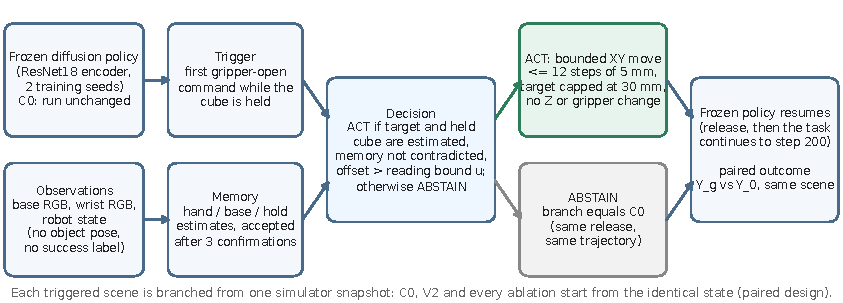
\includegraphics[width=\linewidth]{F2_method.pdf}
\caption{Vision-CENTER V2. At the policy's first gripper-open command while a cube is held, the controller combines current base- and wrist-camera estimates with a confirmed memory of the target cube and of the held cube. It abstains unless both estimates exist, the memory is not contradicted by the current image, and the estimated offset is at least 15\,mm and exceeds its reading bound by at least 10\,mm; otherwise it makes a bounded horizontal move and returns control to the unchanged policy. Every arm is branched from the same simulator snapshot.}\label{fig:method}
\end{figure}

\paragraph{Trigger} The trigger fires at the first control step at which the policy's next queued action opens the gripper directly after at least three consecutive close commands, while the finger opening (sum of the two finger joints) lies between 0.02 and 0.06\,m, i.e.\ the fingers are closed on an object. Only the policy's own action queue and the robot's finger reading are used. At the trigger, the pending release command is held back; if the controller abstains, the queue is released unchanged and the branch is identical to C0.

\paragraph{Observations} The controller receives the base and wrist RGB images ($128\times128$ each), the end-effector (TCP) pose and the finger opening. Cubes are located by colour segmentation and projected with the fixed camera parameters; no model is trained.

\paragraph{Memory} The target cube is often hidden by the held cube at the trigger. V2 therefore keeps three memories, updated from the start of the episode: a \emph{hand} memory (target position from the wrist camera), a \emph{base} memory (target position from the base camera) and a \emph{hold} memory (position of the held cube relative to the gripper, refitted every fourth step while the gripper is closed). A memory entry is used only after $m=3$ consistent observations, and it is dropped when the finger opening changes by more than 1\,mm (hold) or when the current image contradicts it (target). Each estimate carries a reading bound $u$: 2\,mm for the wrist-camera fit, 5\,mm for the base-camera estimate, 2\,mm for the hold fit, and an extra 5\,mm when the gripper was close to the remembered target after its last confirmation.

\paragraph{Decision} Let $\hat{\mathbf{o}}=\hat{\mathbf{x}}_{\mathrm{target}}-\hat{\mathbf{x}}_{\mathrm{held}}$ be the estimated horizontal offset. V2 acts only if
\begin{equation}
\|\hat{\mathbf{o}}\| \;\ge\; 15\ \mathrm{mm} \qquad\text{and}\qquad \|\hat{\mathbf{o}}\| - u \;\ge\; 10\ \mathrm{mm},
\end{equation}
and none of eight abstention rules holds: no held-cube estimate, no target estimate, memory contradicted, held cube too low (carried below 58\,mm, i.e.\ beside rather than above the target), side-contact risk, fewer than 20 steps left, already aligned (first condition violated), or aligned within the reading bound (second condition violated).

\paragraph{Bounded move and hand-back} If V2 acts, it commands horizontal TCP increments $\Delta\mathbf{x}_t$ with
\begin{equation}
\|\Delta\mathbf{x}_t\|\le 5\ \mathrm{mm},\qquad \|\mathbf{x}^{\mathrm{cmd}}_t-\mathbf{x}_{t^\star}\|\le 30\ \mathrm{mm},\qquad t-t^\star\le 12,
\end{equation}
where $\mathbf{x}_t$ is the TCP position, $\mathbf{x}^{\mathrm{cmd}}_t=\mathbf{x}_t+\Delta\mathbf{x}_t$ the commanded position and $\mathbf{x}_{t^\star}$ the TCP position at the trigger, with no vertical and no gripper command, and stops when the re-estimated residual offset is below 10\,mm (5\,mm when the target came from memory) or when the target estimate jumps by more than 3\,mm or the held cube slips by more than 3\,mm. Every step of the move is charged to the 200-step episode budget. The held release command is then passed to the unchanged policy, which continues to the end of the episode. In execution the arm covered about 40\% of each commanded increment (about 2 of 5\,mm per step; Section~\ref{sec:mechanism}), so one move shifts the TCP by at most about 25\,mm and the 30\,mm cap rarely binds; larger offsets cannot be fully corrected by one move.

\paragraph{Ablations and reference} \emph{V1} uses the wrist camera only and no memory. \emph{V2 single frame} uses V2 with $m=1$, so that each estimate rests on the current frame. \emph{V2 without hand/base/hold memory} removes one memory each. \emph{V2 rules off} disables the abstention rules. \emph{Oracle centring} replaces the estimates by the true cube positions and is privileged.

%% ---------------------------------------------------------------------------------------------------------
\section{Experimental protocol}\label{sec:protocol}

\paragraph{Task and simulator} We use \texttt{StackCube-v1} of ManiSkill3 \cite{tao2024maniskill3} (version 3.0.1, commit \texttt{a4a4f92}) on SAPIEN 3.0.3 \cite{xiang2020sapien} with CPU PhysX, a single environment, a Panda arm with a wrist camera, end-effector delta-position control, and a 200-step horizon. Success is the first time the task condition holds (cube A on cube B, static, released); the episode then ends.

\paragraph{Frozen policies} The base policies are RGB diffusion policies \cite{chi2023diffusion} (observation horizon 2, prediction 16, execution 8) with an ImageNet-pretrained ResNet-18 encoder \cite{he2016resnet}, trained on the same 500 motion-planning demonstrations with two training seeds (\emph{policy seed 1} and \emph{policy seed 2}) and frozen before any intervention data were collected. The generalisation study uses a third frozen policy with the original small, non-pretrained convolutional encoder (\emph{PlainConv}).

\paragraph{Splits} Splits are disjoint ranges of scene seeds; all branches of a scene stay in one split.
\begin{itemize}
\item Development (C1): seeds 51100--51299, 200 scenes per policy, all arms.
\item Calibration: seeds 30000--30399, 400 scenes per policy, C0 and V2.
\item Final Test: seeds 90000--90399, 400 scenes per policy, C0 and V2, run once.
\item Generalisation (development level): seeds 51300--51499, PlainConv policy.
\end{itemize}
Before each stage, a placement check confirmed that no new scene repeats a cube placement of any earlier scene (0 identical placements among 2,347 references for calibration and for test).

\paragraph{Pre-registration and freezing} The development stage pre-registered two hypotheses: $H_{\mathrm{gen}}$ (V2 improves on C0 for policy seed 2, which was not used while developing V2) and $H_{\mathrm{mem}}$ (V2 improves on its single-frame variant for both policies, tested as an intersection--union test), with Holm over the two. The candidate (V2 with unchanged constants), the policy family, $\varepsilon$, $\delta$, the tests and all rules were then frozen in a manifest before calibration (SHA-256 \texttt{01b70a06\ldots}). The Final Test manifest (\texttt{94c5a591\ldots}) added the calibration analysis and the environment, and the test runner refused to start unless the live environment matched it (GPU, driver, Python version, upstream commit and the full package list) and three used development scenes reproduced bit for bit the reference recorded on the calibration host.

\paragraph{Hosts} Development ran on a host with NVIDIA driver 550.120. Calibration and the Final Test ran on RTX 4090 hosts with driver 595.99.02. Rendering differs between the two drivers, and with it some policy actions: in 16 of 300 earlier scenes and in 6 of 11 selected diagnostic scenes the outcome differed between hosts. The certificate and the test result therefore refer to the 595.99.02 configuration (Section~\ref{sec:limits}).

\paragraph{Policy sampling noise} The diffusion sampling noise is keyed to the scene and the control step, and is identical for all branches up to the trigger. After a move the policy resumes later and therefore draws different noise than C0 at the same phase of the task, so a discordant pair can reflect policy variance as well as the move. In an earlier development pilot, an arm that only held the robot still for a matched number of steps gave 1 rescue and 1 harm against C0 on 100 scenes; we read this as the approximate size of that floor, not as a correction. The efficacy test compares the deployed system (policy plus controller) with the policy alone and remains valid in this sense.

\paragraph{Role of the AI agent} Experiment orchestration on rented GPU hosts, analysis code, recounts and figure generation were carried out with an AI coding agent (Claude, Anthropic) under the author's direction. Every protocol decision taken during the runs is listed with its approval status in Supplementary Section~S9; the author takes responsibility for all of them.

\paragraph{Recount} All headline numbers were recomputed from the raw scene records, after checking the SHA-256 of every trajectory file, by two implementations (the project code and an independent hand-written count with SciPy); they agreed exactly (Supplementary Section~S8).

%% ---------------------------------------------------------------------------------------------------------
\section{Development results}\label{sec:dev}

\paragraph{Question} On development scenes, does V2 rescue failures without harming successes, and does its memory matter?

\begin{table}[!htbp]
\centering\footnotesize
\caption{Development stage (C1, seeds 51100--51299): successes of 200 scenes, rescues and harms against C0, and number of scenes in which the arm moved. The trigger fired in 195 (seed 1) and 191 (seed 2) scenes. For the oracle the column counts the scenes in which it entered its control loop (every trigger); it actually moved in 93 and 102.}\label{tab:dev}
\resizebox{\linewidth}{!}{\input{\tabdir T2_development_arms.tex}}
\end{table}

\begin{table}[!htbp]
\centering\footnotesize
\caption{Pre-registered development hypotheses (exact one-sided paired tests; Holm over the two hypotheses at $\alpha=0.05$, i.e.\ the smaller p-value is compared with 0.025 and the larger with 0.05; IU = intersection--union).}\label{tab:devtests}
\resizebox{\linewidth}{!}{\input{\tabdir T3_development_tests.tex}}
\end{table}

\paragraph{Evidence} Table~\ref{tab:dev} lists all nine arms. V2 raised success from 171 to 184 (14 rescues, 1 harm) for policy seed 1 and from 164 to 180 (16 rescues, 0 harms) for policy seed 2. The privileged oracle reached 185 and 184. Both pre-registered hypotheses were rejected (Table~\ref{tab:devtests}): V2 against C0 for policy seed 2 ($16$ vs $0$, $p=1.5\times10^{-5}$) and V2 against its single-frame variant for both policies (intersection--union $p=0.0078$).

\begin{figure}[!htbp]
\centering
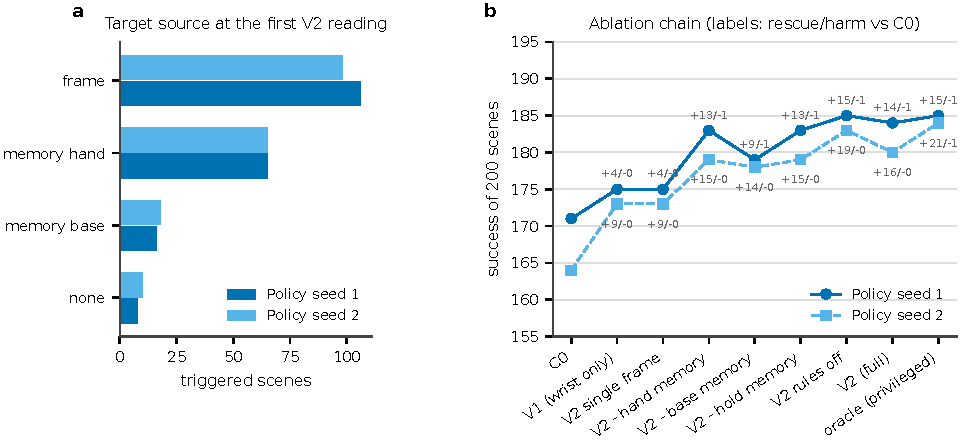
\includegraphics[width=\linewidth]{F4_memory_and_ablation.pdf}
\caption{Memory and ablation on the development scenes. (a) Source of the target estimate at the first V2 reading in triggered scenes: in about one third of them the target came from the wrist-camera memory, because the held cube hid it at the trigger. (b) Successes of all arms; labels give rescues/harms against C0. The single-frame variant behaves like the wrist-only V1, while removing one memory at a time loses less.}\label{fig:memory}
\end{figure}

\paragraph{Interpretation} Figure~\ref{fig:memory}a shows why memory matters: at the first reading the target position came from the current frame in 106 and 98 triggered scenes, from the hand memory in 65 and 65, and from the base memory in 16 and 18; in 8 and 10 there was no target estimate. Without confirmed memory (single frame) the controller acts in 25--30 scenes and rescues 4 and 9; with it, it acts in 39--41 scenes and rescues 14 and 16. Removing only the hand or the hold memory costs one rescue for seed 1 and one for seed 2, while removing the base memory costs five and two, which suggests that the memories partly substitute for each other.

\paragraph{Limits} The single-frame ablation sets the confirmation count to $m=1$, which also changes when a memory entry becomes usable; it is therefore not a pure removal of memory, and $H_{\mathrm{mem}}$ measures the combined effect (Section~\ref{sec:limits}). These are development results on scenes that informed the design; they do not certify a harm rate.

%% ---------------------------------------------------------------------------------------------------------
\section{Calibration certificate and Final Test}\label{sec:confirm}

\paragraph{Question} On new scenes and with nothing changed after development, is the harm rate below 5\%, and does V2 increase success?

\begin{figure}[!htbp]
\centering
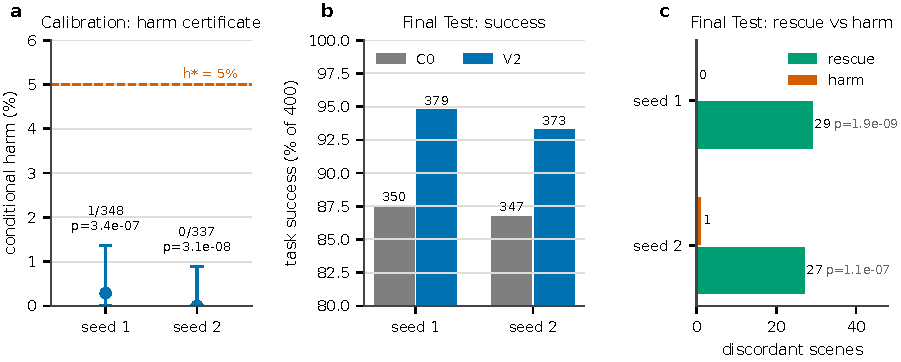
\includegraphics[width=\linewidth]{F3_statistics_calibration_vs_test.pdf}
\caption{Confirmatory stages. (a) Calibration (400 scenes per policy): observed conditional harm with the one-sided 95\% Clopper--Pearson upper bound (descriptive) against the pre-registered level $\varepsilon=5\%$ (marked $h^\ast$); the p-values are those of Eq.~\eqref{eq:cert}. (b) Final Test (400 held-out scenes per policy, run once): task success of C0 and V2. (c) Final Test discordant scenes and the p-values of Eq.~\eqref{eq:eff}.}\label{fig:stats}
\end{figure}

\begin{table}[!htbp]
\centering\footnotesize
\caption{Calibration certificate and Final Test. Trig.: scenes with a trigger; Acted: scenes in which V2 moved; C0, V2: successes of 400. Calibration tests $h(g)\le 0.05$ (Eq.~\ref{eq:cert}); the Final Test tests efficacy (Eq.~\ref{eq:eff}); both with Holm over the two policies at level 0.05.}\label{tab:confirm}
\resizebox{\linewidth}{!}{\input{\tabdir T4_calibration_and_test.tex}}
\end{table}

\paragraph{Evidence: calibration} V2 turned 1 of 348 (policy seed 1) and 0 of 337 (policy seed 2) baseline successes into failures (Table~\ref{tab:confirm}, Fig.~\ref{fig:stats}a). The exact p-values were $3.4\times10^{-7}$ and $3.1\times10^{-8}$, far below the Holm thresholds, so the joint statement ``$h(g)\le0.05$ for both policies'' holds at $\delta=0.05$. As descriptive quantities, the one-sided 95\% Clopper--Pearson upper bounds \cite{clopper1934} of the conditional harm are 1.36\% and 0.89\%. V2 moved in 73 and 66 scenes; among the baseline successes in which it moved, it caused 1 harm in 48 and 0 in 36. Because abstaining and untriggered branches equal C0 by construction, harm can occur only where V2 moves, so much of the margin of the certificate comes from abstention. Restricted to the baseline successes in which V2 moved, the one-sided 95\% Clopper--Pearson upper bounds are 9.5\% and 8.0\% (post hoc; on the test split 0/38 and 1/46, 7.6\% and 9.9\%). The certificate is therefore a statement about the deployed system, the policy together with its gated controller, not about the move alone. The level $\varepsilon=5\%$ was fixed at the start of the project; it corresponds to about 17 lost successes out of 348, more than half of the rescue gain observed in development. The success counts of calibration (348 to 371 and 337 to 366) were pre-declared as descriptive and are not used as evidence of efficacy.

\paragraph{Evidence: Final Test} The Final Test ran once, after a separate approval, with the frozen manifest verified before and after the run. Success rose from 350 to 379 (87.5\% to 94.75\%) for policy seed 1 and from 347 to 373 (86.75\% to 93.25\%) for policy seed 2. The discordant scenes were 29 rescues and 0 harms ($p=1.9\times10^{-9}$) and 27 rescues and 1 harm ($p=1.1\times10^{-7}$), so both efficacy nulls were rejected under Holm (Fig.~\ref{fig:stats}b,c). A paired bootstrap of the success difference (20,000 resamples; post hoc and descriptive) gives 95\% intervals of $[+4.8, +10.0]$ and $[+4.0, +9.0]$ percentage points. Harm on the test scenes was 0 of 350 and 1 of 347; the harm guarantee itself rests on the calibration certificate, not on these counts.

\paragraph{Interpretation} The gain and the low harm seen in development carried over to 1,600 new paired scenes, without any change to the controller. Pooled over both policies and the test split, the four cells were 696 both-succeed, 56 rescues, 1 harm and 47 both-fail scenes (Fig.~\ref{fig:problem}a).

\paragraph{Limits} The guarantee concerns the scene distribution $\mathcal{D}$ of this task, the two policies, and the simulator configuration of the calibration host. Calibration and test did not reproduce development outcomes exactly because of the host difference; one pre-declared smoke criterion (bit-identity with the development records) was therefore not met (Section~\ref{sec:limits}).

%% ---------------------------------------------------------------------------------------------------------
\section{Mechanism: how a rescue and a harm happen}\label{sec:mechanism}

\paragraph{Question} Which steps of the chain observation $\to$ memory $\to$ decision $\to$ move $\to$ hand-back produce rescues, and where does harm enter?

\paragraph{Rescue} In the typical rescue (Fig.~\ref{fig:problem}b) the policy carries the cube to a position beside the target and is about to release it there. V2 estimates the offset, moves the gripper towards the target, and the policy's own release then places the cube on the target. Across all 715 acted branches of all arms in development, the movement direction agreed with the command: after the first step, the cosine between the actual and the commanded horizontal displacement was at least 0.9 in every branch (Fig.~\ref{fig:control}c).

\begin{figure}[!htbp]
\centering
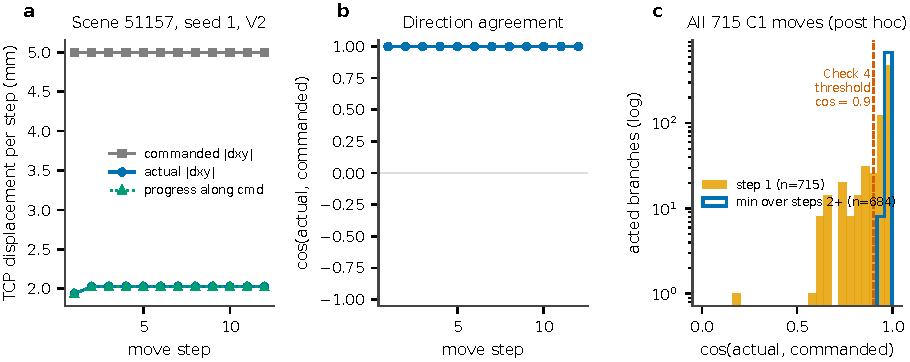
\includegraphics[width=\linewidth]{F6_control_check4.pdf}
\caption{Commanded versus actual motion. (a,b) Scene 51157, V2: commanded and actual horizontal TCP displacement per move step and their direction cosine. (c) All 715 acted branches in development (post hoc): the first step often deviates in direction because the arm is still moving with the policy's previous command (110 branches below the pre-declared 0.9 threshold); from the second step on, no branch falls below it.}\label{fig:control}
\end{figure}

\begin{figure}[!htbp]
\centering
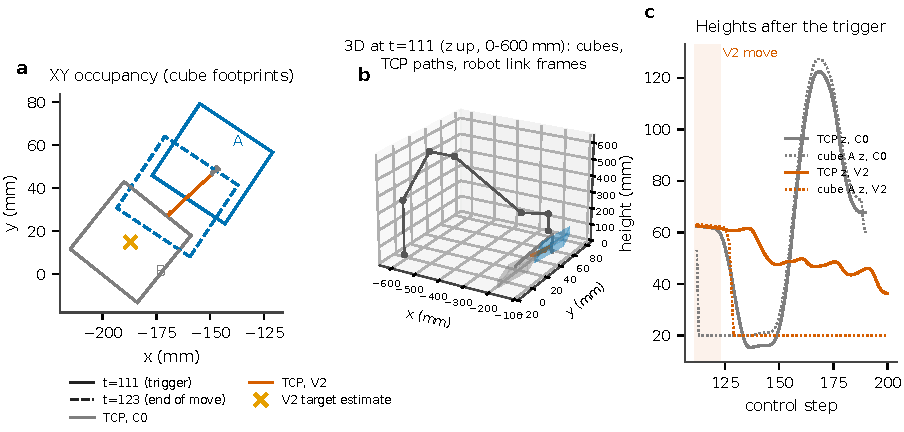
\includegraphics[width=\linewidth]{F5_spatial_51157.pdf}
\caption{The harm case 51157 (policy seed 1, development). (a) Footprints of the held cube A (blue) and target cube B (grey) at the trigger (solid) and at the end of the V2 move (dashed), the TCP paths and the target estimate. (b) Three-dimensional view at the trigger: cube boxes from the logged poses, TCP paths of C0 (grey) and V2 (orange), and the robot link frames. (c) Heights of the TCP and of cube A after the trigger.}\label{fig:spatial}
\end{figure}

\paragraph{Harm} The single development harm of V2 for policy seed 1 (scene 51157) is instructive because V2 did what it was designed to do. At the trigger the held cube was 54.6\,mm from the target centre; the V2 estimate was 54.7\,mm (error 0.15\,mm), within its 9\,mm reading bound. V2 moved for the full 12 steps and reduced the true offset to 30.4\,mm (Fig.~\ref{fig:spatial}a). The move tracked its direction but not its length: each 5\,mm command produced about 2\,mm of TCP displacement (Fig.~\ref{fig:control}a,b), so the 30\,mm cap was not reached. The policy then released the cube beside the target, it fell to the table, and the policy did not regrasp it before the horizon (Fig.~\ref{fig:spatial}c). Without V2 the policy also dropped the cube, but it regrasped it and completed the stack at step 190, 10 steps before the horizon; the 12 steps spent on the move exceed that margin. The record therefore supports two contributing factors, an incomplete correction and the time budget, without separating them. Acting on an offset larger than one move can correct is a weakness of the design: among acted scenes with an estimated offset above 40\,mm there were 3 in development (1 rescue, 1 harm, the latter being 51157), none in calibration, and 8 in the Final Test (6 rescues and 1 harm, the only harm of the test).

\paragraph{The pre-declared motion check} A pre-declared check (``Check 4'') required every move step to have direction cosine $\ge0.9$ and progress $\ge0.2$\,mm. It failed in 9 of 41 V2 moves (seed 1) and 5 of 39 (seed 2). In all 14 failures, only the first step failed and only on direction (cosine 0.63--0.88); the later steps of the same moves had cosine 0.934--0.999. We keep the official FAIL and read it as a first-step lag of the arm, not as a wrong move direction.

\paragraph{Missed rescues} The oracle rescued 15 and 21 development scenes; V2 rescued 14 and 16. Of the oracle rescues, V2 missed 1 (policy seed 1) and 5 (policy seed 2), all by abstaining: side-contact risk (2), held cube carried too low (2), no target estimate (1) and aligned within the reading bound (1). These rules were set to avoid moves on missing or uncertain estimates; in these scenes they cost a rescue. Supplementary Section~S3 lists every abstention reason.

\paragraph{Limits} The mechanism is read from development records (driver 550.120) and is descriptive; it is not a causal decomposition. The 51157 case is one scene, and its C0 branch has a different outcome on the calibration host, so the mechanism describes the development configuration rather than the certified one.

%% ---------------------------------------------------------------------------------------------------------
\section{Validity of the physical record}\label{sec:physics}

\paragraph{Question} The mechanism analysis uses logged contacts, distances and poses. Are these measurements trustworthy, and does any failure change a result?

\begin{table}[!htbp]
\centering\footnotesize
\caption{Measurement-validity checks on the development record (post hoc unless stated). S4--S6 were declared before the analysis; their official status is kept.}\label{tab:physics}
\input{\tabdir T5_physics_validity.tex}
\end{table}

\paragraph{Checks} We defined three checks before analysing the record (Table~\ref{tab:physics}). \emph{S4}: during a move, the minimum distance between robot geometry and the target cube stays positive. \emph{S5}: reconstructed penetrations between bodies do not exceed 1\,mm. \emph{S6}: for each contact pair listed by PhysX, the logged separation agrees with the gap we reconstruct from the logged poses and collision shapes within 1\,mm.

\paragraph{Evidence} S4 failed in one of 715 acted branches, an oracle branch ($-2.16$\,mm, policy seed 2, scene 51152), and in none of the V2 branches. S5 failed in two short events with fast-moving cubes (11 of 3,874 branch records: 400 trunks plus 9 arms in each of 386 triggered scene-runs). Replacing every logged collision mesh by its convex hull changed no S4 or S5 status (Fig.~\ref{fig:hull}). S6 \emph{failed}: 54,267 of 580,539 listed pair rows (9.3\%) disagreed by more than 1\,mm (Fig.~\ref{fig:s6}a).

\begin{figure}[!htbp]
\centering
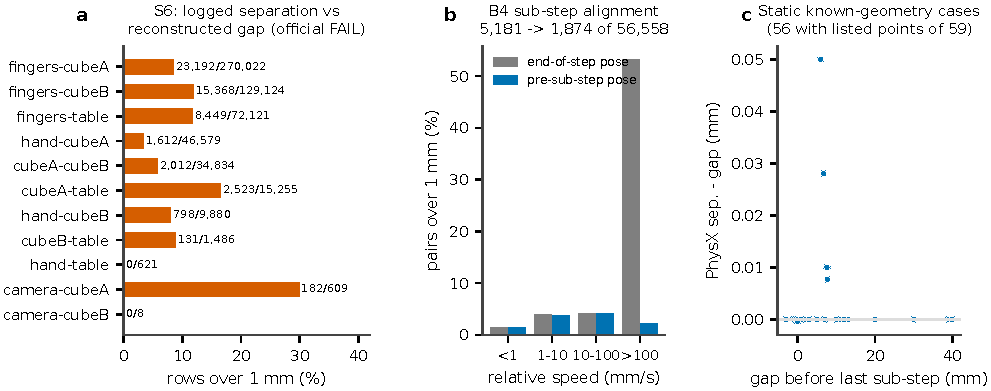
\includegraphics[width=\linewidth]{F7_physics_s6_b4.pdf}
\caption{Contact-separation check S6. (a) Rows over 1\,mm by pair kind (official FAIL). (b) Logging every physics sub-step on 11 used scene-runs: comparing with the pose before the last sub-step removes most disagreements of fast pairs. (c) Static boxes with known geometry: the PhysX separation equals the analytic gap before the last sub-step within 0.05\,mm.}\label{fig:s6}
\end{figure}

\paragraph{Partial explanation} Three follow-up measurements explain part of the S6 failure. First, on static box pairs with known geometry, the PhysX separation equals the analytic gap before the last sub-step within 0.05\,mm (Fig.~\ref{fig:s6}c), which fixes the definition of the logged quantity \cite{nvidia_physx_contact}. Second, logging every sub-step of 11 used scene-runs (re-run on the calibration host) showed that the contact list is computed at the pose before the last of the five sub-steps of a control step; comparing with that pose reduced the disagreements above 1\,mm from 5,181 to 1,874 of 56,558 pairs, and for pairs faster than 100\,mm/s from 3,436 to 146 (Fig.~\ref{fig:s6}b). Third, the remaining 1,874 rows are all zero-impulse proximity pairs between a finger box and a cube; shape-index mismatch and static edge geometry were excluded as causes. Their origin is not established.

\begin{figure}[!htbp]
\centering
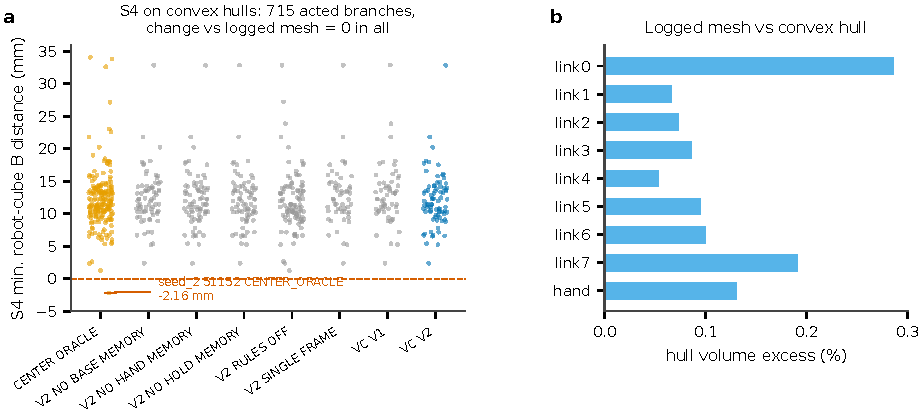
\includegraphics[width=\linewidth]{F8_hull_sensitivity.pdf}
\caption{Collision-geometry sensitivity. (a) S4 minimum robot--target distance on convex hulls for all 715 acted branches; the change with respect to the logged meshes is zero in every branch, and the only negative value is an oracle branch. (b) Volume excess of the convex hull over the logged mesh per link (at most 0.3\%).}\label{fig:hull}
\end{figure}

\paragraph{Interpretation} The task outcomes, the harm certificate and the efficacy test use only the success flag of each branch, which the simulator computes from its own state; they do not depend on S4--S6. The S6 failure limits the use of logged separations for fine-grained contact analysis, which is why we use them only descriptively.

\paragraph{Limits} S6 keeps its official FAIL status. No check here establishes continuous-time collision freedom; a contact between control steps can be missed.

%% ---------------------------------------------------------------------------------------------------------
\section{A second policy architecture}\label{sec:generalization}

\paragraph{Question} Is the gain specific to the ResNet-18 policies on which V2 was developed?

\begin{figure}[!htbp]
\centering
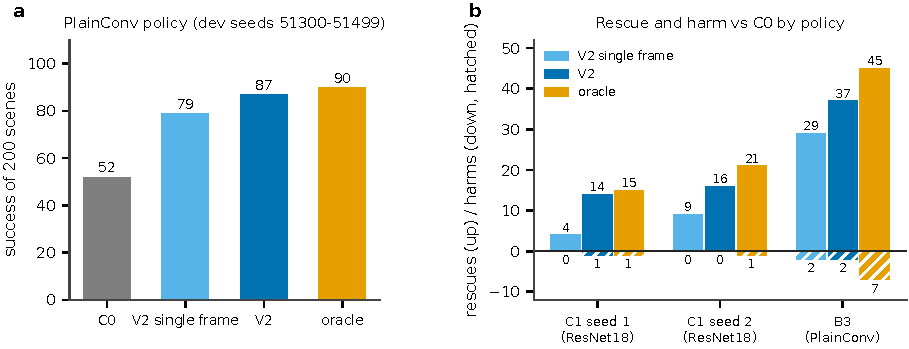
\includegraphics[width=\linewidth]{F9_generalization_plainconv.pdf}
\caption{Unchanged V2 on a frozen policy of a different architecture (PlainConv encoder; development seeds 51300--51499). (a) Successes of 200 scenes. (b) Rescues (up) and harms (down, hatched) against C0 for the development policies and the PlainConv policy.}\label{fig:gen}
\end{figure}

\begin{table}[!htbp]
\centering\footnotesize
\caption{PlainConv policy, development level (200 scenes; 95\% Clopper--Pearson intervals).}\label{tab:gen}
\input{\tabdir T6_generalization_plainconv.tex}
\end{table}

\paragraph{Evidence} Applied without any change to a frozen policy with a weaker, non-pretrained encoder, V2 raised success from 52 to 87 of 200 scenes, with 37 rescues and 2 harms ($p=1.4\times10^{-9}$, one pre-declared test; Table~\ref{tab:gen}, Fig.~\ref{fig:gen}). It recovered 37 of the 45 oracle rescues; the oracle itself caused 7 harms. The single-frame variant reached 79 (29 rescues, 2 harms).

\paragraph{Interpretation and limits} The same release-time offset is a dominant failure mode for a weaker policy, and, at development level, V2 corrects it without retuning. This is a development-level result on one task: there is no calibration certificate for this policy, and its 2 harms among 52 baseline successes (3.8\%) are not a bound. The two architectures share the task and the demonstrations, so this is not evidence of transfer to other tasks.

%% ---------------------------------------------------------------------------------------------------------
\section{Discussion}\label{sec:discussion}

\paragraph{Separating rescue from harm changes what is reported} A success rate of 94.75\% versus 87.5\% does not tell a user whether the intervention ever breaks a working episode. The paired four-cell count does: on the Final Test, 1 of 697 baseline successes was lost while 56 of 103 failures were rescued. The certificate turns the calibration counterpart of this statement into a bound with a stated error probability, although most of its margin comes from scenes in which V2 does not move.

\paragraph{Abstention as a precaution} V2 acted in about one in five triggered scenes (41 of 195 and 39 of 191 in development). Most triggered scenes were already aligned, and in the rest V2 abstained whenever an estimate was missing or contradicted. The rules-off ablation acted in 53 and 50 development scenes instead of 41 and 39 and gained one and three rescues, and had the same harms (1 and 0). The development data therefore do not show that the rules reduce harm; we kept them as a precaution before the confirmatory stages.

\paragraph{Harm through time and incomplete motion} The observed harm mechanism was not a collision but a combination of an under-tracking move and a spent time budget. Commanding 5\,mm per step produced about 2\,mm, so a correction that the controller believed sufficient was not. A recovery that reads its own executed displacement, or that charges fewer steps to the episode, could reduce both effects; this was not tested.

\paragraph{What the memory does} Memory let V2 act when the target was hidden. Because the ablation that removes it also changes the confirmation count, our data support the statement that the confirmed multi-frame estimate improves on a single-frame estimate, not that memory alone does.

%% ---------------------------------------------------------------------------------------------------------
\section{Limitations}\label{sec:limits}

\begin{itemize}
\item \textbf{One task, simulation only.} All results are for \texttt{StackCube-v1} with rendered images. There is no real-robot experiment, and nothing is claimed about other tasks.
\item \textbf{Statistical, task-level guarantee.} The certificate bounds the probability of turning a baseline success into a failure on the calibration distribution. It is not a guarantee of physical safety, force limits or collision freedom, and the physics checks do not establish continuous-time collision safety.
\item \textbf{Measurement validity.} The contact-separation check S6 failed (9.3\% of rows) and remains failed; on the 11 sub-step-logged scene-runs, 3.3\% of listed separated pairs remain unexplained after sub-step alignment.
\item \textbf{Host configuration.} Development ran on driver 550.120 and the confirmatory stages on driver 595.99.02. Outcomes differed between hosts in some scenes, so development estimates are linked to the confirmatory results only qualitatively. The certificate and the test result refer to the 595.99.02 configuration.
\item \textbf{Deviation from a pre-declared criterion.} Before calibration, a smoke run was required to reproduce the development records bit for bit. It did not, because of the host difference; the runner did reproduce the unchanged development collector on the same host. The decision to proceed on a fixed host type was recorded and committed before the first calibration rollout, by the AI agent that ran the experiment, without a separate approval by the author at that time; the author reviewed it afterwards and takes responsibility for it. Nothing about the candidate, the policies, the levels or the tests changed.
\item \textbf{Memory ablation confound.} The single-frame variant changes both the use of earlier frames and the confirmation count.
\item \textbf{No external baseline and policy-noise floor.} The comparators are the uninterrupted policy, ablations and a privileged oracle; no learned recovery or retry baseline was run. Part of the discordance may be policy variance after the resumption (Section~\ref{sec:protocol}).
\item \textbf{Two policies of one family} for the certificate, and a single PlainConv policy at development level for generalisation.
\end{itemize}

%% ---------------------------------------------------------------------------------------------------------
\section{Conclusion}\label{sec:conclusion}

A recovery intervention on a frozen policy can rescue failures and can also destroy successes; the two should be measured separately. With paired branching from a common snapshot, an exact binomial certificate on a calibration split and a single held-out confirmatory test, an observation-only release-time centring controller was certified (exact test, $\delta=0.05$, calibration-host configuration) to have a conditional harm rate of at most 5\% for two diffusion policies and to raise their success from 87.5\% to 94.75\% and from 86.75\% to 93.25\% on new scenes. The descriptive mechanism analysis traces a representative rescue and the single development harm to measurable steps of the controller, and the audit of the physical record states which measurements can be trusted. The same protocol can be applied to other recovery interventions; whether this controller transfers to other tasks or to a real robot remains open.

%% ---------------------------------------------------------------------------------------------------------
\section*{CRediT authorship contribution statement}
\textbf{[Author name to confirm]:} Conceptualization, Methodology, Software, Investigation, Formal analysis, Data curation, Visualization, Writing -- original draft, Writing -- review \& editing. [To be confirmed by the author.]

\section*{Declaration of competing interest}
[To be confirmed by the author.] The author declares that they have no known competing financial interests or personal relationships that could have appeared to influence the work reported in this paper.

\section*{Funding}
[To be confirmed by the author.] This research did not receive any specific grant from funding agencies in the public, commercial, or not-for-profit sectors.

\section*{Data availability}
[To be confirmed by the author.] The scene records, analysis code, figure and table generators, and SHA-256 manifests are available from the author's repository [link to be added]; raw trajectory archives (about 14\,GB) are available on request.

\section*{Declaration of generative AI and AI-assisted technologies in the manuscript preparation process}
[Draft; to be confirmed by the author.] During the preparation of this work the author used Claude (Anthropic) to write and run analysis code, draft text, and generate figures from the recorded data. After using this tool, the author reviewed and edited the content as needed and takes full responsibility for the content of the published article.

\bibliographystyle{elsarticle-num}
\bibliography{references}

\end{document}
